\documentclass[12pt]{article}
\usepackage{../preamble3}
%\pagenumbering{gobble}
\title{Math Miscellani}
\author{James \& Patrick}
\date{Revised:~\today}

\begin{document}
\maketitle
\begin{minipage}{\textwidth}
\maketitle
\begin{abstract}
This note reviews tips and tricks and selected problems to prepare for middle school math competitions.
\end{abstract}
\end{minipage}

\thispagestyle{empty}
\clearpage
\addtocounter{page}{-1}

\section*{Geometry}

%%%%%%%%%%%%%%%%%%%%%%%%%%%%%%%%%%%%%%%%%%%%%%%%%%%%%%%%%%%%%%%%%%%%%%%%
\subsection*{Triangle}
Height and Area of an equilateral triangle with side $a$.

\begin{answer}
\begin{tikzpicture}\node[textbox]{%
    \begin{minipagex}{\dimexpr\textwidth-20pt}
        Let $A$ denote the area, and $h$ the height of the triangle. 
        \begin{center}
        \begin{tikzpicture}[thick, sharp corners, inner sep=1mm, outer sep =1mm, scale=4]
        \draw (0,0) -- (0.5,0) node[midway,below]{$a/2$} -- (1,0) -- (0.5, 0.866) -- cycle node[midway,left]{$a$}; 
        \draw[dashed] (0.5,0) -- (0.5,0.866) node[midway,right]{$h$};
        \end{tikzpicture}
        \end{center}
        The area of the triangle is given by one-half the product of the base and height:
        \begin{align*}
        A = \frac{1}{2} ah
        \end{align*}
        The height $h$ is unknown, but can be found by an application of the Pythagoras theorem.
        \begin{align*}
        & h^2 + \left(\frac{a}{2}\right)^2 = a^2 \\
        \Rightarrow
        h^2 & = a^2 - \frac{a^2}{4} 
              = \frac{3a^2}{4}
        \end{align*}
        And thus,
        \begin{empheq}[box={\mathbox[colback=white]}]{equation*}
            h = \frac{a}{2} \sqrt{3}
        \end{empheq}
        \begin{empheq}[box={\mathbox[colback=white]}]{equation*}
            A = \left(\frac{a}{2}\right)^2 \sqrt{3}
        \end{empheq}
    \end{minipagex}
    };
\end{tikzpicture}%
\end{answer}
%%%%%%%%%%%%%%%%%%%%%%%%%%%%%%%%%%%%%%%%%%%%%%%%%%%%%%%%%%%%%%%%%%%%%%%%

\newpage

%%%%%%%%%%%%%%%%%%%%%%%%%%%%%%%%%%%%%%%%%%%%%%%%%%%%%%%%%%%%%%%%%%%%%%%%
\subsection*{From Words to Equations}
There were $9$ adults and $11$ children at the movie at $11{:}45$a.m. By $11{:}50$a.m., $7$ more adults and $8$ more children were at the movie. At $12{:}00$p.m., there were $60$ adults and children, and the ratio of adults to children was the same as at $11{:}45$a.m. How many more children came to the movie between $11{:}50$a.m. and $12{:}00$p.m.?

\begin{answer}
\begin{tikzpicture}\node[textbox]{%
    \begin{minipagex}{\dimexpr\textwidth-20pt}
        Let $a$ denote the number of adults and $c$ denote the number of children, who came to the movie between $11{:}50$a.m. and $12{:}00$p.m.
        \begin{align*}
        a + c & = 25 \\
        \frac{a + 16}{c + 19} & = \frac{9}{11}
        \end{align*}
        This is a system of two equations in two unknowns, $a$ and $c$. After a simple transformation, the second equation becomes linear in $a$ and $c$.
        \begin{align*}
        a + c & = 25 \\
        11 (a + 16) & = 9 (c + 19) \Rightarrow 11a - 9c = 9 \cdot 19 - 11 \cdot 16
        \end{align*}
        Since we are interested in solving for $c$, let's substitute $a$ out:
        \begin{align*}
        11 (25-c) - 9c & = 9 \cdot 19 - 11 \cdot 16 \\
        \Rightarrow 
        c & = \frac{11 \cdot 25 + 11 \cdot 16 - 9 \cdot 19}{20} 
            = \frac{11 \cdot 41 - 9 \cdot 19}{20} 
            = \frac{410 + 41 - 190 + 19}{20} \\
          & = \frac{280}{20} = 14 \\
        \Rightarrow 
        a & = 25 - 14 = 11
        \end{align*}        
        \begin{empheq}[box={\mathbox[colback=white]}]{equation*}
            11 ~\text{children}
        \end{empheq}
    \end{minipagex}
    };
\end{tikzpicture}%
\end{answer}
%%%%%%%%%%%%%%%%%%%%%%%%%%%%%%%%%%%%%%%%%%%%%%%%%%%%%%%%%%%%%%%%%%%%%%%%

\newpage

%%%%%%%%%%%%%%%%%%%%%%%%%%%%%%%%%%%%%%%%%%%%%%%%%%%%%%%%%%%%%%%%%%%%%%%%
\subsection*{Quadratic Equations}
The sum of a number $x$ and its reciprocal equals $-\dfrac{17}{4}$. What is the sum of all possible values of $x$? Express your answer as a common fraction. 

\begin{answer}
\begin{tikzpicture}\node[textbox]{%
    \begin{minipagex}{\dimexpr\textwidth-20pt}
        The possible values of $x$ satisfy:
        \begin{align*}
        x + \frac{1}{x} = -\frac{17}{4}
        \end{align*}
        This is a quadratic equation in disguise. Multiply through by $x$:
        \begin{align*}
        x^2 + 1 = -\frac{17}{4} x
        \end{align*}
        Rearrange to obtain the standard display format:
        \begin{align*}
        x^2 + \left(\sfrac{17}{4}\right) x + 1 = 0
        \end{align*}
        To find the values of $x$, we would solve this equation. One approach is to apply the well-known formula for the quadratic equation. Let's review the formula:
        \begin{align*}
        ax^2 + bx + c = 0 
        \Rightarrow
        x = \frac{-b \pm \sqrt{b^2-4ac}}{2a}
        \end{align*}
        Now substitute the values $a=1$, $b=\sfrac{17}{4}$, and $c=1$ into the above formula.
        
        However, this is not needed. The question asks for the ``sum of all possible values of $x$''. Quadratic equation generally have two solutions (but note that these solutions could be complex / a solution could appear twice). Let $r_1$ and $r_2$ denote the roots (\textit{aka} solutions) of a quadratic equation. The roots clearly solve the following equation:
        \begin{align*}
        (x-r_1)(x-r_2) = 0
        \end{align*}
        Distributing the product and rearranging yields:
        \begin{align*}
        x^2 -(r_1+r_2)x + r_1 r_2 = 0
        \end{align*}
        Or, to put it in words:
        \begin{align*}
        \text{$X^2$ minus (sum)~$X$ plus (product)} = 0
        \end{align*}
        And thus we can read the answer to the question straight out of the equation. Just beware of the negative sign in front of the sum-of-roots term. 
        \begin{empheq}[box={\mathbox[colback=white]}]{equation*}
            \text{sum of the roots}~ = -\frac{17}{4}
        \end{empheq}
    \end{minipagex}
    };
\end{tikzpicture}%
\end{answer}
%%%%%%%%%%%%%%%%%%%%%%%%%%%%%%%%%%%%%%%%%%%%%%%%%%%%%%%%%%%%%%%%%%%%%%%%

\newpage

%%%%%%%%%%%%%%%%%%%%%%%%%%%%%%%%%%%%%%%%%%%%%%%%%%%%%%%%%%%%%%%%%%%%%%%%
\subsection*{Mean Cats}
The mean number of cats living in each of the $50$ apartments in a particular apartment building is $0.44$ cats. A total of $32$ apartments in the building are cat-free. What is the mean number of cats in the apartments that have at least one cat? Express your answer to the nearest tenth. 

\begin{answer}
\begin{tikzpicture}\node[textbox]{%
    \begin{minipagex}{\dimexpr\textwidth-20pt}
        Let $n$ denote the total number of cats. The mean number of cats over $50$ apartments is
        \begin{align*}
        \frac{n}{50} = 0.44 
        \Rightarrow 
        n = 50 \times 0.44 = 22
        \end{align*}
        There are therefore $22$ cats living in $18$ apartments ($50-32=18$). The mean over those $18$ apartments is:
        \begin{align*}
        \frac{22}{18} = 1.22\ldots
        \end{align*}        
        \begin{empheq}[box={\mathbox[colback=white]}]{equation*}
            1.2 ~\text{cats}
        \end{empheq}
    \end{minipagex}
    };
\end{tikzpicture}%
\end{answer}
%%%%%%%%%%%%%%%%%%%%%%%%%%%%%%%%%%%%%%%%%%%%%%%%%%%%%%%%%%%%%%%%%%%%%%%%

\newpage

%%%%%%%%%%%%%%%%%%%%%%%%%%%%%%%%%%%%%%%%%%%%%%%%%%%%%%%%%%%%%%%%%%%%%%%%
\subsection*{Mean Grades}
The mean of Danielle's test scores is $85$. If Danielle's lowest test score, which is $61$ were to be discarded, the mean of her remaining test scores would be $88$. How many tests did Danielle take?

\begin{answer}
\begin{tikzpicture}\node[textbox]{%
    \begin{minipagex}{\dimexpr\textwidth-20pt}
        Let $n$ denote the total number of tests she took. Let $s$ denote the sum of all her scores. Danielle's mean score when all scores are included is:
        \begin{align*}
        \frac{s}{n} = 85
        \end{align*}
        Danielle's mean score when the lowest grade is excluded is:
        \begin{align*}
        \frac{s-61}{n-1} = 88
        \end{align*}
        This yields a linear system of two equations in two unknowns $s$ and $n$:
        \begin{align*}
        s - 85n & = 0 \\
        s - 88n  + 27 & = 0
        \end{align*}
        Since we want to solve for $n$, we'll substitute $s$ from the first equation into the second:
        \begin{align*}
        85n - 88n  + 27 = 0 \Rightarrow 3n = 27 \Rightarrow n = 9
        \end{align*}
        \begin{empheq}[box={\mathbox[colback=white]}]{equation*}
            9 ~\text{tests}
        \end{empheq}
    \end{minipagex}
    };
\end{tikzpicture}%
\end{answer}
%%%%%%%%%%%%%%%%%%%%%%%%%%%%%%%%%%%%%%%%%%%%%%%%%%%%%%%%%%%%%%%%%%%%%%%%

\newpage

%%%%%%%%%%%%%%%%%%%%%%%%%%%%%%%%%%%%%%%%%%%%%%%%%%%%%%%%%%%%%%%%%%%%%%%%
\subsection*{Rotated Square}
The vertices of the smaller square in the figure are at trisection points of the sides of the larger square. What is the ratio of the area of the smaller square to the area of the larger square? Express your answer as a common fraction.

\begin{minipage}[b]{\linewidth}
\centering
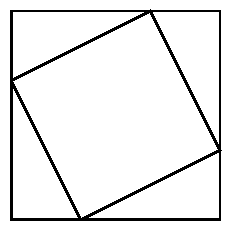
\includegraphics[height=5cm]{square-rotated}
\end{minipage}


\begin{answer}
\begin{tikzpicture}\node[textbox]{%
    \begin{minipagex}{\dimexpr\textwidth-20pt}
        If the larger square has side measuring $a$ units, its area is $a^2$. If the smaller square has side measuring $x$ units, its area is $x^2$. Since the side of the smaller square is the hypotenuse of the inscribed triangle, we have
        \begin{align*}
        x^2 = \left(\frac{a}{3}\right)^2 + \left(\frac{2a}{3}\right)^2 
            = \left(\frac{a}{3}\right)^2 (1 + 2^2) 
            = \frac{5}{9} a^2 
        \end{align*}
        \begin{empheq}[box={\mathbox[colback=white]}]{equation*}
            \frac{\text{outer square}}{\text{inscribed square}} = \frac{5}{9}
        \end{empheq}
    \end{minipagex}
    };
\end{tikzpicture}%
\end{answer}
%%%%%%%%%%%%%%%%%%%%%%%%%%%%%%%%%%%%%%%%%%%%%%%%%%%%%%%%%%%%%%%%%%%%%%%%

\newpage

%%%%%%%%%%%%%%%%%%%%%%%%%%%%%%%%%%%%%%%%%%%%%%%%%%%%%%%%%%%%%%%%%%%%%%%%
\subsection*{Area of a Quadrilateral}
Quadrilateral $PSTU$ is inscribed in semicircle $O$, as shown, with $PQ=3$ units, $QR=5$ units and $RS=4$ units. What is the area of quadrilateral $PSTU$? Express your answer as a decimal to the nearest tenth. 

\begin{minipage}[b]{\linewidth}
\centering
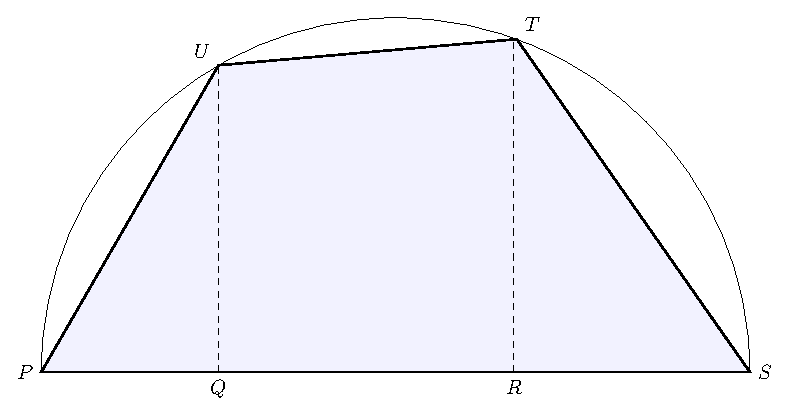
\includegraphics[height=2.5cm]{quadrilateral-inscribed}
\end{minipage}
\begin{answer}
\begin{tikzpicture}\node[textbox]{%
    \begin{minipagex}{\dimexpr\textwidth-20pt}
        One approach to calculating the area of quadrilateral $PUTS$ is to divide it into triangle $PQU$, triangle $SRT$, and trapezoid $QUTR$. A trapezoid is a quadrilateral with only one pair of parallel sides. To compute these areas, we need the heights $h_1$ and $h_2$. To calculate $h_1$, apply the Pythagoras theorem to triangle $OQU$. And likewise $h_2$ with triangle $ORT$. 
        \begin{minipage}[b]{\linewidth}
        \centering
        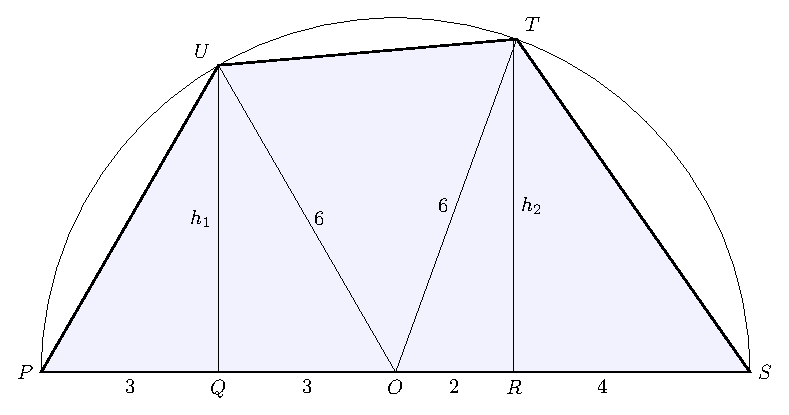
\includegraphics[height=5cm]{quadrilateral-inscribed-labeled}
        \end{minipage}
        \begin{align*}
        h_1 & = \sqrt{6^2 -3^2} = \sqrt{27} = 3\sqrt{3} \approx 5.196 \\
        h_2 & = \sqrt{6^2 -2^2} =\sqrt{32} = 4\sqrt{2} \approx 5.657
        \end{align*}
        The area of triangle $PQU$ and $SRT$ are:
        \begin{align*}
        \frac{1}{2} \times 3 \times h_1 & = 4.5\sqrt{3} \approx 7.794 \\
        \frac{1}{2} \times 4 \times h_2 & = 8\sqrt{2} \approx 11.314 
        \end{align*}
        The area of trapezoid $QUTR$ equals the area of a parallelogram with equal base and height equal to the average height. 
        \begin{align*}
        QR \times \frac{h_1+h_2}{2} 
          = 5 \times \frac{3\sqrt{3}+4\sqrt{2}}{2}
          = 10\sqrt{2} + 7.5\sqrt{3}
          \approx 27.133 
        \end{align*}
        Adding up the areas of the triangles and trapezoid yields:
        \begin{align*}
        4.5\sqrt{3} + 8\sqrt{2} + 7.5\sqrt{3} + 10\sqrt{2}
          = 18\sqrt{2} + 12\sqrt{3}
          \approx 46.240
        \end{align*}
        \begin{empheq}[box={\mathbox[colback=white]}]{equation*}
            46.2~\text{units}^2
        \end{empheq}
    \end{minipagex}
    };
\end{tikzpicture}%
\end{answer}
%%%%%%%%%%%%%%%%%%%%%%%%%%%%%%%%%%%%%%%%%%%%%%%%%%%%%%%%%%%%%%%%%%%%%%%%

\newpage

%%%%%%%%%%%%%%%%%%%%%%%%%%%%%%%%%%%%%%%%%%%%%%%%%%%%%%%%%%%%%%%%%%%%%%%%
\subsection*{Median in a Range}
What is the median of the integers between $1$ and $1000$ that are divisible by $28$?

\begin{answer}
\begin{tikzpicture}\node[textbox]{%
    \begin{minipagex}{\dimexpr\textwidth-20pt}
        There are $35$ integers divisible by $28$ in the range $[1,1000]$, since
        \begin{align*}
        \frac{1000}{28} \approx 35.7
        \end{align*}
        Since the number of integers divisible by $28$ is odd, their median is equal to the $18$th element, which is $504$, since
        \begin{align*}
        18 \times 28 = 504
        \end{align*}
        \begin{empheq}[box={\mathbox[colback=white]}]{equation*}
            504
        \end{empheq}
    \end{minipagex}
    };
\end{tikzpicture}%
\end{answer}
%%%%%%%%%%%%%%%%%%%%%%%%%%%%%%%%%%%%%%%%%%%%%%%%%%%%%%%%%%%%%%%%%%%%%%%%

\newpage

%%%%%%%%%%%%%%%%%%%%%%%%%%%%%%%%%%%%%%%%%%%%%%%%%%%%%%%%%%%%%%%%%%%%%%%%
\subsection*{Median in a Range}
What is the median of the integers between $1$ and $1000$ that are \textit{not} divisible by $28$?

\begin{answer}
\begin{tikzpicture}\node[textbox]{%
    \begin{minipagex}{\dimexpr\textwidth-20pt}
        Take the range $[1,1000]$ as a starting point and consider the effect of removing the multiples of $28$. The median of the integers in the range $[1,1000]$, including the multiples of $28$, is
        \begin{align*}
        \frac{1000+1}{2} = 500.5
        \end{align*}
        There are $35$ integers divisible by $28$ in the range $[1,1000]$, of which $17$ are below the median and $18$ are above, since
        \begin{align*}
        \frac{1000}{28} \approx 35.7, ~~
        \frac{500}{28} \approx 17.9
        \end{align*}
        A single deletion below the median shifts the median upwards by half a unit, while a single deletion above the median shifts it downwards by half a unit.  Removing the multiples of $28$ results in $17$ deletions below and $18$ deletions above, for an overall shift downwards of half a unit. The new median is therefore
        \begin{align*}
        500.5 - 0.5 = 500
        \end{align*}        
        \begin{empheq}[box={\mathbox[colback=white]}]{equation*}
            500
        \end{empheq}
    \end{minipagex}
    };
\end{tikzpicture}%
\end{answer}
%%%%%%%%%%%%%%%%%%%%%%%%%%%%%%%%%%%%%%%%%%%%%%%%%%%%%%%%%%%%%%%%%%%%%%%%


\newpage

%%%%%%%%%%%%%%%%%%%%%%%%%%%%%%%%%%%%%%%%%%%%%%%%%%%%%%%%%%%%%%%%%%%%%%%%
\subsection*{Mystery Sum}
If $2015=101a+19b$, for positive integers $a$ and $b$, what is the value of $a+b$?

\begin{answer}
\begin{tikzpicture}\node[textbox]{%
    \begin{minipagex}{\dimexpr\textwidth-20pt}
        In complete desperation, we tried different values of $a$ until we got a hit, but there has to be a trick. To be continued...
        \begin{align*}
        2015 = 101 \times 16 + 19 \times 21 \\
        \Rightarrow 
        a = 16, b = 21
        \Rightarrow 
        a + b = 16 + 21 = 37
        \end{align*}        
        \begin{empheq}[box={\mathbox[colback=white]}]{equation*}
            37
        \end{empheq}
    \end{minipagex}
    };
\end{tikzpicture}%
\end{answer}
%%%%%%%%%%%%%%%%%%%%%%%%%%%%%%%%%%%%%%%%%%%%%%%%%%%%%%%%%%%%%%%%%%%%%%%%

\newpage

%%%%%%%%%%%%%%%%%%%%%%%%%%%%%%%%%%%%%%%%%%%%%%%%%%%%%%%%%%%%%%%%%%%%%%%%
\subsection*{Mystery Integer}
What positive four-digit integer has its thousands and hundreds digits add up to the tens digit, its hundreds and tens digits add up to its ones digit and its tens and ones digits add up to the two-digit number formed by the thousands and hundreds digits?

\begin{answer}
\begin{tikzpicture}\node[textbox]{%
    \begin{minipagex}{\dimexpr\textwidth-20pt}
        Let $a$, $b$, $c$, $d$ denote the digits of the integers $abcd$, where
        \begin{align*}
        1 \leq a \leq 9, ~ 0 \leq b \leq 9, ~ 0 \leq c \leq 9, ~0 \leq d \leq 9
        \end{align*} 
        The text translates to the following set of three equations.
        \begin{align*}
        a + b & = c \\
        b + c & = d \\
        c + d & = 10a + b
        \end{align*}
        While these equations are linear, there are only $3$ equations for $4$ unknowns, so some clever guessing must be brought to bear on the problem. Since $a>0$ (otherwise it would not be a $4$-digit integer), the third equation implies
        \begin{align*}
        c + d & \geq 10
        \end{align*}
        In some sense, the sum $c+d$ is `large'. Meanwhile the second equation suggests that $d$ is likely to be greater than $c$ (only if $b=0$ that would not be true). So we will start to guess from $d=9$ and move down to $d=8$, $d=7$, and so on, until we hit on a solution. Thus, if $d=9$, we have:
        \begin{align*}
        a + b & = c \\
        b + c & = 9 \\
        c + 9 & = 10a + b \\
        \Rightarrow a = 1, b = 4, c = 5, d = 9
        \end{align*}
        We hit a solution on our first attempt!
        \begin{empheq}[box={\mathbox[colback=white]}]{equation*}
            1459
        \end{empheq}
    \end{minipagex}
    };
\end{tikzpicture}%
\end{answer}
%%%%%%%%%%%%%%%%%%%%%%%%%%%%%%%%%%%%%%%%%%%%%%%%%%%%%%%%%%%%%%%%%%%%%%%%


\end{document}

